\section{Introduction}

% The evolution toward Artificial General Intelligence (AGI) is constrained by the complex physical world, demanding that cognitive abilities of Large-Scale Models (LMs) toward the heterogeneous multimodal world representation. as it leads the academic community to develop more advanced algorithms to push the boundaries of their abilities, including understanding, synthesis, and reasoning. % 句子太长了
% However, the physical world is composed of low-level and fragmented foundational information, and perceiving its underlying logic from this information is the most complex and challenging task for LMs because it requires high-level cognitive ability, which integrates multiple single cognitive abilities. 
% Therefore, the High-Level Cognition (HLC) task was first proposed by Liu et al. \cite{liu2025can}. 
% To concretize the process of solving this task, the models are required to first understand low-level information, then synthesize this fragmented information, and finally perform reasoning to obtain high-level conclusions.
% Meanwhile, these abilities are pushed to their boundaries in this process.
% They explored it using information in the textual modality and demonstrated that LLMs lack this ability because the HLC task cannot be effectively solved.
% Nevertheless, a viable solution was discovered by them: the gradient optimization-based parameter fine-tuning strategy can endow LLMs with HLC, thereby improving their performance on this task to some extent.
% However, this strategy is essentially data-driven statistical fitting.
% Although its effectiveness has been validated in the textual modality, foundational information exists in multiple modalities in the physical world.
% Therefore, a scientific problem emerges: Does the HLC endowed by fine-tuning reflect an intrinsic and modality-agnostic ability to perceive the physical world, or is it a product of statistical fitting that depends on semantic associations embedded in natural language through shortcut learning?

\begin{figure}[!t]
	\centering
	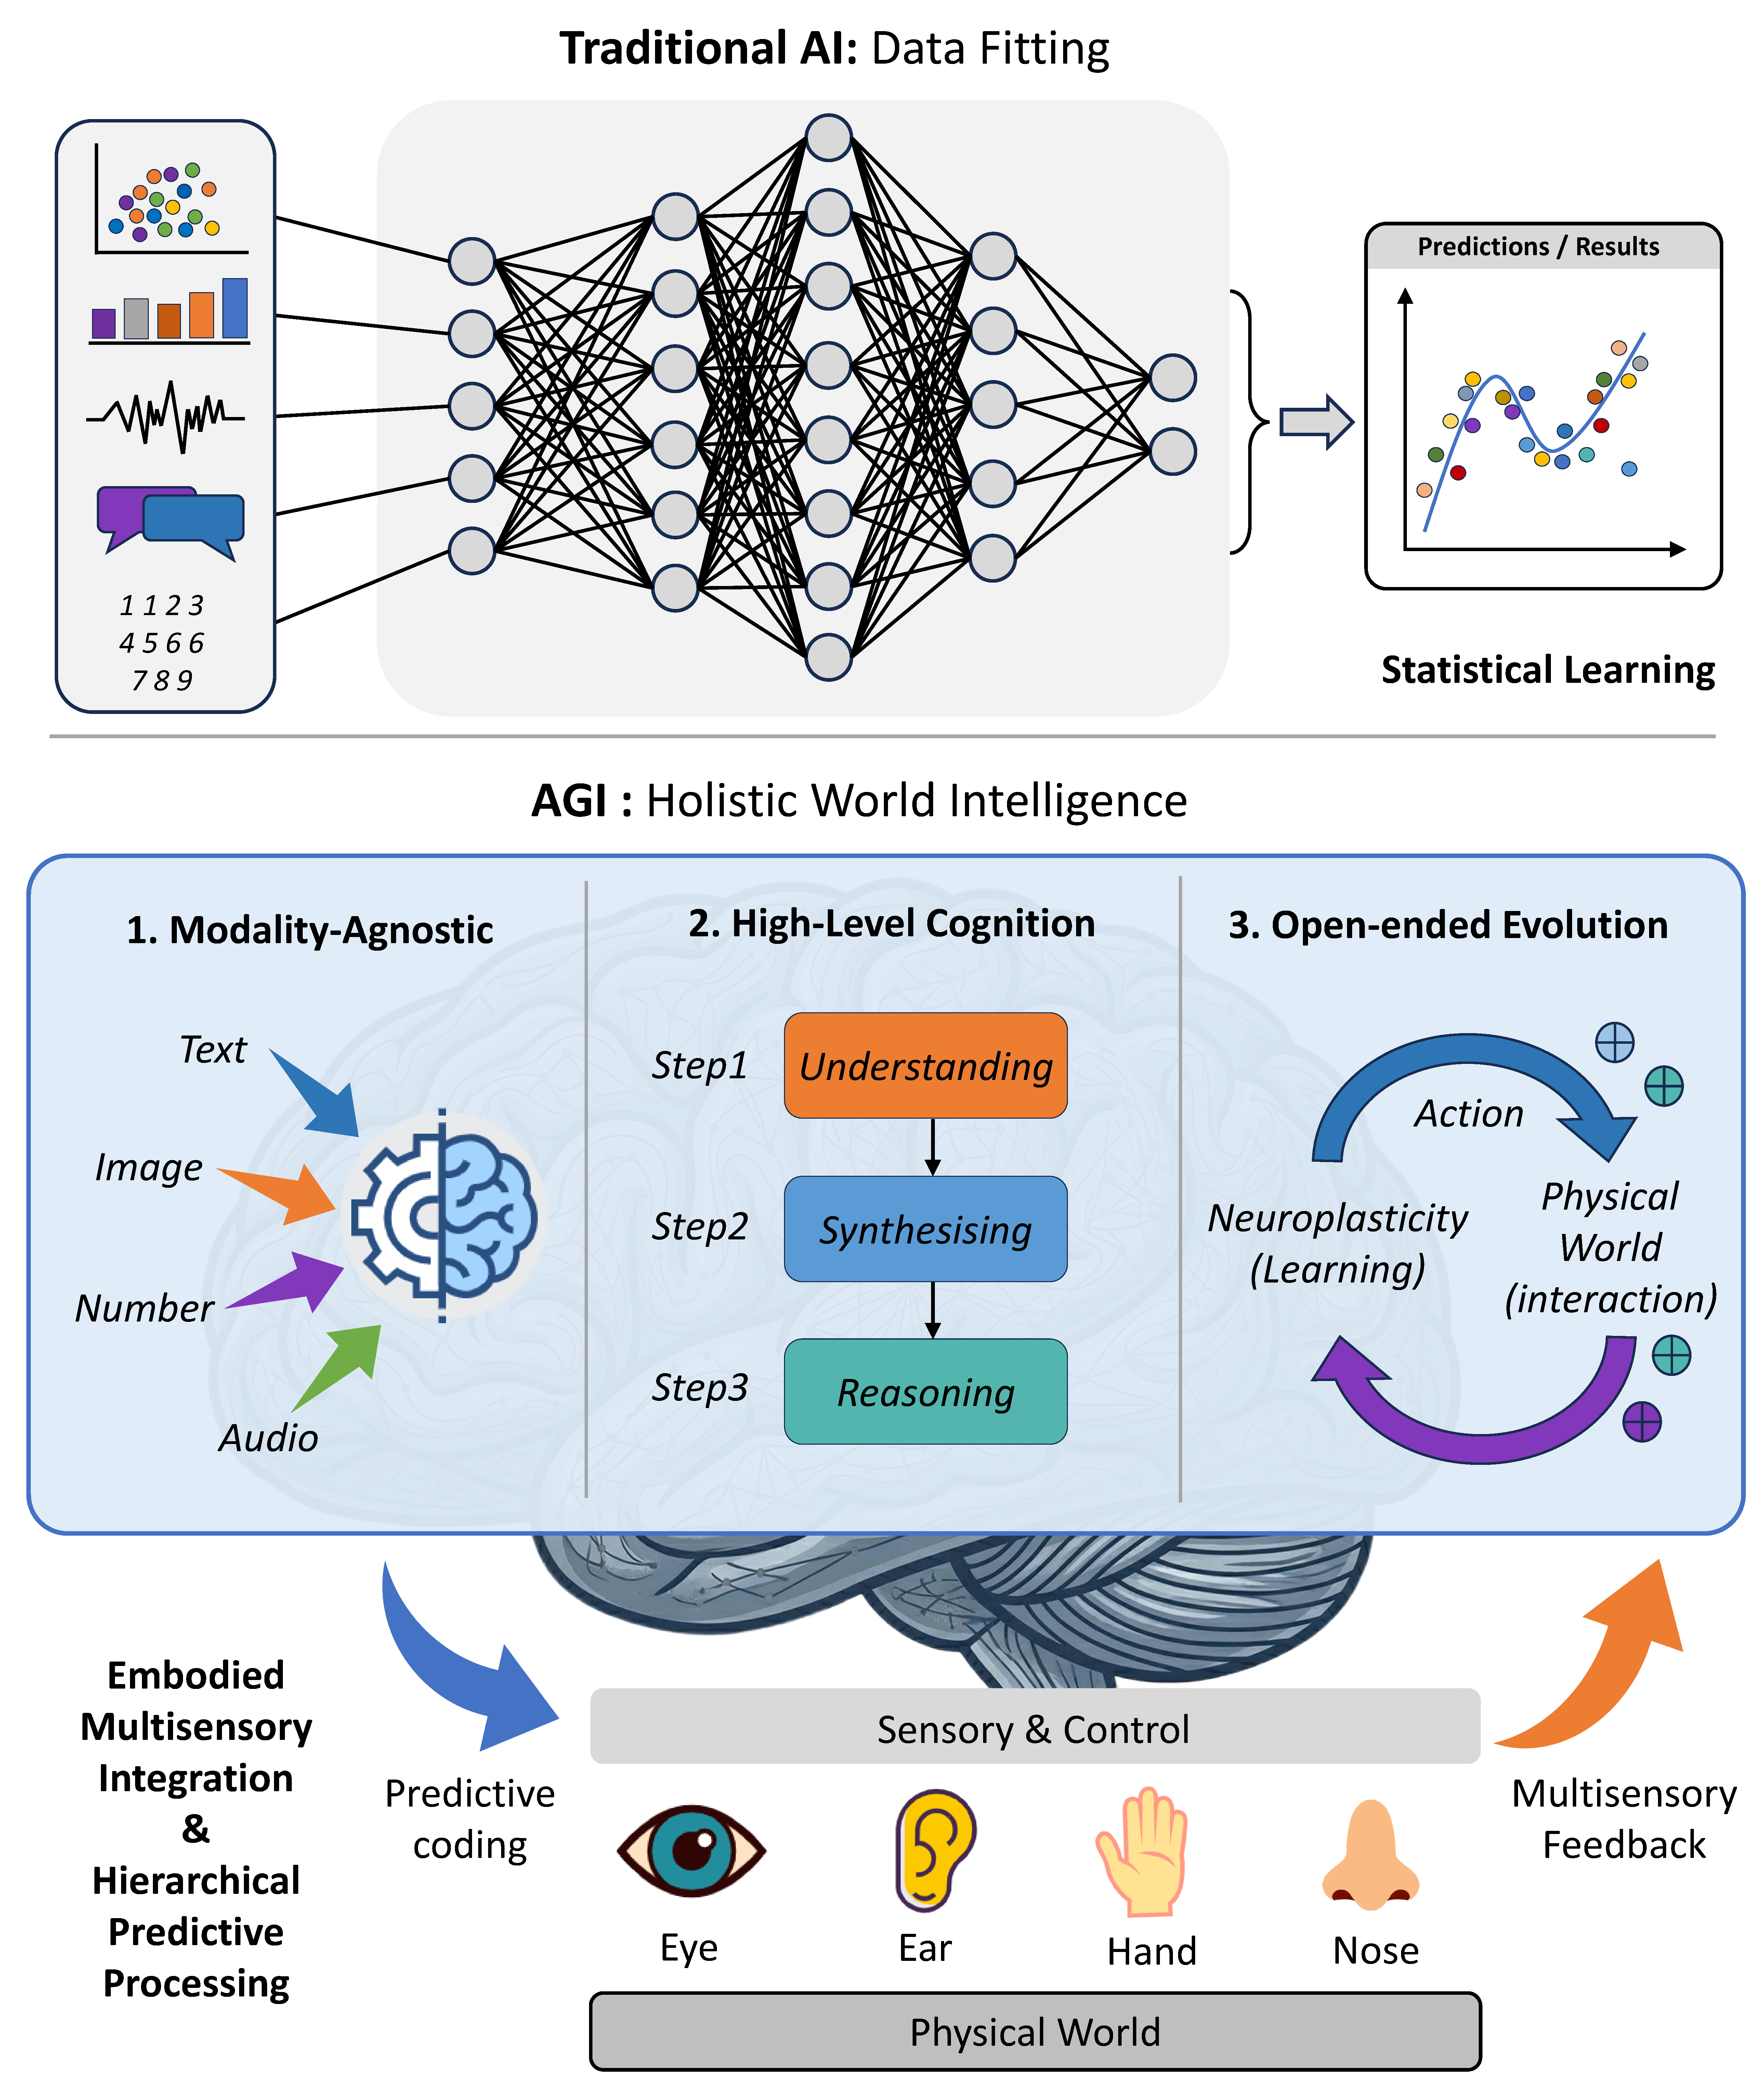
\includegraphics[scale=0.1]{figure/figure1.pdf}
	\caption{An illustration of our work. LMs can be endowed with HLC in the textual modality, but experience a Cognitive Collapse in the numerical and visual modalities. }
	\label{figure1}
\end{figure}

% To address this, the task should be further extended from the textual modality. While human knowledge is primarily recorded in text, the underlying logic of the physical world is driven by continuous and non-semantic numerical values (e.g., sensor readings, spatiotemporal coordinates, and statistical logs) and spatial topologies without explicit semantic entities (e.g., heatmaps and trajectory maps). These data are the essential medium to verify whether the intrinsic ability to perceive the physical world is possessed by models directly, stripped of their linguistic shells. Accordingly, the task is extended to numerical and visual modalities in this paper, and the Multimodal High-Level Cognition (MHLC) task is proposed. Unlike traditional numerical modality tasks, where fitting precision or data forecasting are focused, and traditional visual modality tasks, where object detection or image classification are emphasized, the MHLC task challenges models to perceive the underlying logic of the physical world from low-level numerical and spatial topologies, where direct extraction or mapping is impossible and multiple cognitive abilities are required. Specifically, these non-semantic data are first pushed to the boundaries of understanding (e.g., the meaning and connections of these numbers or topologies), then an implicit global framework is formed by pushing these fragmented data to the boundaries of synthesizing (e.g., the state, trend, and distribution in numerical values, or the spatial perspective, relational graph and structural map in spatial topologies). Finally, high-level conclusions can be obtained by pushing this implicit global framework to the boundaries of reasoning. This process is completely devoid of semantic cues. If the success of HLC in previous textual-modality work comes from mastery of general physical-world perception, this ability should theoretically be reproduced in numerical and visual modalities.

% However, existing multimodal datasets are not suitable for evaluating this task because they are limited to low-level mechanical processing of numbers or images. Their ground truth is still an extension of the same type of low-level features (e.g., time-series forecasting, discrete visual labels), lacking annotations for high-level logic. To bridge this gap, a new multimodal benchmark dataset \textit{MatchIntel2} is constructed in this paper. As a cross-modality counterpart to previous textual-modality HLC research, it collects real-time statistical numerical sequences and player-position visual heatmaps from thousands of professional soccer matches as low-level and fragmented foundational information, while expert-annotated team playing styles are treated as high-level conclusions.

% Based on this dataset, the MHLC of current state-of-the-art Large-scale Models (LMs), including LLMs and Vision-Language Models (VLMs), is evaluated in numerical and visual modalities. The experimental results show a thought-provoking phenomenon: a \textit{Cognitive Collapse} is observed in these models when they solve the MHLC task. Specifically, even after parameter-efficient supervised fine-tuning, the performance of these models with massive parameter scales on the MHLC task remains at random level. Contrary to the success of textual-modality HLC in previous work, this phenomenon indicates that the HLC endowed by gradient optimization-based parameter fine-tuning is highly dependent on semantic associations embedded in natural language, and once semantic assistance is removed, it fails to be established. Moreover, an interesting finding is that supervised-trained lightweight models with negligible parameters achieve superior performance on the MHLC task, which suggests that the design of specialized model architectures plays a more crucial role than mere parameter scale in achieving MHLC. Figure \ref{figure1} shows an illustration of this paper.

% The main contributions of this paper are summarized as follows:
% \begin{itemize} 
% 	\item{}The MHLC task is proposed. To complement the modality of previous HLC task research, the task is extended from the textual modality to the numerical and visual modalities. It provides a more comprehensive evaluation framework for exploring the HLC of LMs on multiple modalities.
% 	\item{}A new multimodal benchmark dataset \textit{MatchIntel2} is constructed. It contains low-level information and high-level conclusions about soccer matches from both numerical and visual modalities, which bridges the gap in the multimodal evaluation of HLC, and provides a more rigorous experimental benchmark for exploring the MHLC of LMs.
% 	\item{}The modality limitations of current LMs in deriving HLC are revealed. Experimental results show that the fine-tuned models still perform at the random level on MHLC tasks, even though their HLC can be effectively endowed in the textual modality by the same strategy. In contrast, superior performance is achieved by trained lightweight models with negligible parameters. This demonstrates that endowed textual HLC is a product of statistical fitting via semantic shortcuts, rather than an intrinsic and modality-agnostic ability. These findings further clarify the cognitive boundaries of LMs in the physical world and highlight the importance of specialized architectures.
% \end{itemize}

% The organization of the remaining sections is as follows: related work is reviewed in Section~\ref{sec:related}; the MHLC task formulation together with the MatchIntel2 benchmark is introduced in Section~\ref{sec:mhlc-benchmark}; main experiments together with a surface-level collapse severity analysis are presented in Section~\ref{sec:experiment}; Section~\ref{sec:discussion} develops the MHLC collapse narrative, U/S/R decomposition, ablations that rule out shallow explanations (prompting and scaling), and future directions toward multimodal AGI-relevant cognition; conclusions are summarized in Section~\ref{sec:conclusion}.

The evolution of Artificial General Intelligence (AGI) is constrained by the complex physical world, necessitating that Large-scale Models (LMs) develop a Gestalt World-Level Capability (GWC) to effectively process heterogeneous real-world representations. Drawing inspiration from Embodied Multisensory Integration and Hierarchical Predictive Processing within cognitive neuroscience, we posit that the GWC must encompass three core characteristics. First, this capability must be Modality-Agnostic, as humans transcend representational barriers to resolve complex, multimodal physical scenarios utilizing unified neural representations. Second, it must demonstrate High-level Cognition, given that the advanced cognitive hierarchy of the human brain is fundamentally a chain-like thinking process integrating diverse foundational cognitive functions. Finally, it must facilitate Open-ended Evolution, enabling the model to continuously refine and augment its capabilities through ongoing learning and environmental interaction, analogous to human neuroplasticity.

However, existing approaches exhibit fundamental flaws in realizing these objectives. First, current Multimodal Large Language Models (MLLMs) inherently rely on merely aligned semantic spaces, lacking a unified representation of the physical world’s multidimensional properties. Second, existing plug-and-play reasoning paradigms are essentially internal logical deductions driven by externally designed rules, rather than endogenous, autonomously driven cognitive structures. Third, fitting methods or evolutionary algorithms that rely purely on massive datasets are fundamentally interpolating static snapshots of the physical world, unable to interact dynamically with the environment for continuous capability augmentation. Consequently, achieving GWC remains a formidable challenge.

Overcoming this hindered by deficiencies across three dimensions. In terms of Structured Frameworks, the absence of Gestalt World Representation datasets, metrics, and benchmarks precludes precise GWC measurement. Regarding Analytical Mechanisms, a lack of theoretical guidance consigns internal mechanisms to a black box, making GWC uninterpretable. Methodologically, a dearth of novel Paradigms to trigger endogenous logical growth and continuous physical interaction prevents GWC enhancement.

To this end, our contributions are summarized as follows: 
\begin{itemize} 
	\item{}We propose the first comprehensive Framework for GWC, including a benchmark and evaluation protocol, providing infrastructure to measure this capability emergence under heterogeneous representations. 
	\item{}We conduct an in-depth empirical investigation revealing the phenomenon of Capability Collapse in current models when processing complex multimodal physical data, filling a gap in theoretical analysis. 
	\item{}We deeply analyze the fundamental causes of high-level cognitive limitations, offering crucial guidance for overcoming evolutionary stagnation and designing next-generation architectures genuinely equipped with GWC.
\end{itemize}

